
\subsection{Font-Format}
\emph{Italic} \\
\textbf{Bold} \\
\texttt{Code} \\
Tabstops: Eins \quad Zwei \quad Drei

\subsection{Kommentare}
(siehe Code)
%Kommentare

\subsection{Mathematische Ausdrücke}
Bruch: $\dfrac{a}{b}$ \\
Vektor: $\dbinom{n}{k}$ \\
Wurzel: $\sqrt{2}$ \\
Potenz: $2^{2}$ \\
Summe: $\sum_{n=1}^{\infty} 2^{-n} = 1$ \\
Limes: $\lim_{x\to\infty} f(x)$

\subsection{Bilder}
\begin{figure}[h]
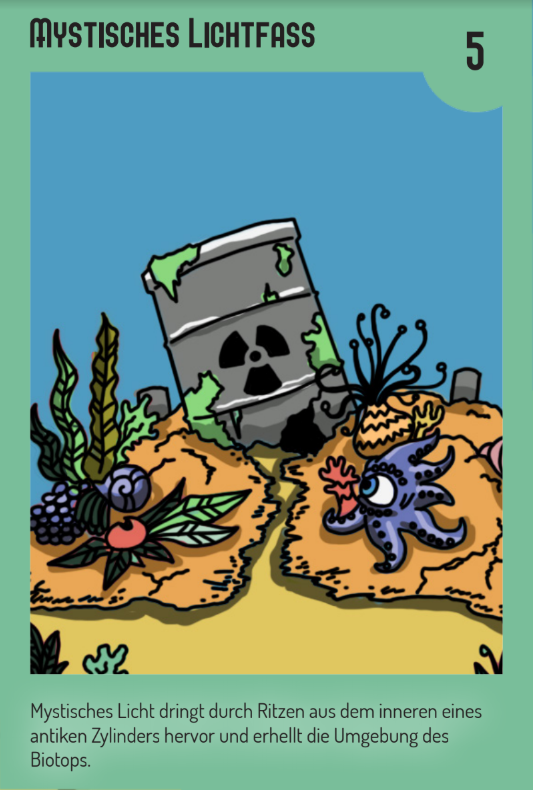
\includegraphics[width=0.2\textwidth]{../img/demo_img.PNG}
\caption{Mystisches Lichtfass}
\label{fig:mystisches_lichtfass}
\end{figure}
Und so referenziert man dynamisch auf die Abbildung \figref{mystisches_lichtfass}

\subsection{Zitate und Referenzen}
So zitiert man mit Referenz \cite[Seite 100]{Test1}
